%% BioMed_Central_Tex_Template_v1.06
%%                                      %
%  bmc_article.tex            ver: 1.06 %
%                                       %

%%IMPORTANT: do not delete the first line of this template
%%It must be present to enable the BMC Submission system to
%%recognise this template!!

%%%%%%%%%%%%%%%%%%%%%%%%%%%%%%%%%%%%%%%%%
%%                                     %%
%%  LaTeX template for BioMed Central  %%
%%     journal article submissions     %%
%%                                     %%
%%          <8 June 2012>              %%
%%                                     %%
%%                                     %%
%%%%%%%%%%%%%%%%%%%%%%%%%%%%%%%%%%%%%%%%%


%%%%%%%%%%%%%%%%%%%%%%%%%%%%%%%%%%%%%%%%%%%%%%%%%%%%%%%%%%%%%%%%%%%%%
%%                                                                 %%
%% For instructions on how to fill out this Tex template           %%
%% document please refer to Readme.html and the instructions for   %%
%% authors page on the biomed central website                      %%
%% http://www.biomedcentral.com/info/authors/                      %%
%%                                                                 %%
%% Please do not use \input{...} to include other tex files.       %%
%% Submit your LaTeX manuscript as one .tex document.              %%
%%                                                                 %%
%% All additional figures and files should be attached             %%
%% separately and not embedded in the \TeX\ document itself.       %%
%%                                                                 %%
%% BioMed Central currently use the MikTex distribution of         %%
%% TeX for Windows) of TeX and LaTeX.  This is available from      %%
%% http://www.miktex.org                                           %%
%%                                                                 %%
%%%%%%%%%%%%%%%%%%%%%%%%%%%%%%%%%%%%%%%%%%%%%%%%%%%%%%%%%%%%%%%%%%%%%

%%% additional documentclass options:
%  [doublespacing]
%  [linenumbers]   - put the line numbers on margins

%%% loading packages, author definitions

%\documentclass[twocolumn]{bmcart}% uncomment this for twocolumn layout and comment line below
\documentclass{bmcart}

%%% Load packages
%\usepackage{amsthm,amsmath}
%\RequirePackage{natbib}
%\RequirePackage{hyperref}
\usepackage[utf8]{inputenc} %unicode support
%\usepackage[applemac]{inputenc} %applemac support if unicode package fails
%\usepackage[latin1]{inputenc} %UNIX support if unicode package fails


% Load packages
\usepackage{url}  % Formatting web addresses  
\usepackage{hhline}
\usepackage{xspace}
%\usepackage{graphicx}
%\usepackage{authblk}

\newif\iffiginline
\figinlinefalse

%%%%%%%%%%%%%%%%%%%%%%%%%%%%%%%%%%%%%%%%%%%%%%%%%
%%                                             %%
%%  If you wish to display your graphics for   %%
%%  your own use using includegraphic or       %%
%%  includegraphics, then comment out the      %%
%%  following two lines of code.               %%
%%  NB: These line *must* be included when     %%
%%  submitting to BMC.                         %%
%%  All figure files must be submitted as      %%
%%  separate graphics through the BMC          %%
%%  submission process, not included in the    %%
%%  submitted article.                         %%
%%                                             %%
%%%%%%%%%%%%%%%%%%%%%%%%%%%%%%%%%%%%%%%%%%%%%%%%%


\def\includegraphic{}
\def\includegraphics{}


%%% Put your definitions there:
\startlocaldefs
\endlocaldefs

% Begin ...
\begin{document}



\newcommand{\forexample}{e.g.\@\xspace}
\newcommand{\thatis}{i.e.\@\xspace}
\newcommand{\andothers}{et al.\@\xspace}
\newcommand{\kmer}{\ensuremath{k}-mer\xspace}
\newcommand{\kmers}{\ensuremath{k}-mers\xspace}
\newcommand{\tool}{Lighter\xspace}
\newcommand{\ecoli}{\emph{E. coli}\xspace}

\newcommand\myworries[1]{\textcolor{red}{#1}}%\usepackage[applemac]{inputenc} %applemac support if unicode package fails

%%% Start of article front matter
\begin{frontmatter}

\begin{fmbox}
\dochead{Software}
%%%%%%%%%%%%%%%%%%%%%%%%%%%%%%%%%%%%%%%%%%%%%%
%%                                          %%
%% Enter the title of your article here     %%
%%                                          %%
%%%%%%%%%%%%%%%%%%%%%%%%%%%%%%%%%%%%%%%%%%%%%%

%\title{A Probablistic Space-efficient Method of Obtaining Solid Kmers with An Appliction of Error Correction}
\title{Lighter: fast and memory-efficient error correction without counting}

%%%%%%%%%%%%%%%%%%%%%%%%%%%%%%%%%%%%%%%%%%%%%%
%%                                          %%
%% Enter the authors here                   %%
%%                                          %%
%% Specify information, if available,       %%
%% in the form:                             %%
%%   <key>={<id1>,<id2>}                    %%
%%   <key>=                                 %%
%% Comment or delete the keys which are     %%
%% not used. Repeat \author command as much %%
%% as required.                             %%
%%                                          %%
%%%%%%%%%%%%%%%%%%%%%%%%%%%%%%%%%%%%%%%%%%%%%%


%\author[1,2]{Li Song}
%\author[2,1]{Liliana Florea}
%\author[1,2]{Ben Langmead\thanks{langmea@cs.jhu.edu}}
%\affil[1]{Department of Computer Science, Johns Hopkins University}
%\affil[2]{McKusick-Nathans Institute of Genetic Medicine, Johns Hopkins University School of Medicine}

\author[
	addressref={aff1},
	email={lsong10@jhu.edu}
]{\inits{L}\fnm{Li} \snm{Song} }
\author[
	addressref={aff2, aff1},
	email={florea@jhu.edu}
]{\inits{L}\fnm{Liliana} \snm{Florea}}
\author[
	addressref={aff1, aff2},
	corref={aff1},
	email={langmea@cs.jhu.edu}
]{\inits{B}\fnm{Ben} \snm{Langmead}}


%\renewcommand\Authands{ and }


%\author{Li Song$^1$
 % Liliana Florea$^2$
 % Ben Langmead$^3$
%}

%%%%%%%%%%%%%%%%%%%%%%%%%%%%%%%%%%%%%%%%%%%%%%
%%                                          %%
%% Enter the authors' addresses here        %%
%%                                          %%
%% Repeat \address commands as much as      %%
%% required.                                %%
%%                                          %%
%%%%%%%%%%%%%%%%%%%%%%%%%%%%%%%%%%%%%%%%%%%%%%
\address[id=aff1]{%                           % unique id
  \orgname{Department of Computer Science, Johns Hopkins University}, % university, etc
  %\street{Waterloo Road},                     %
  \postcode{21218},                                % post or zip code
  \city{Baltimore},                              % city
  \cny{USA}                                    % country
}
\address[id=aff2]{%
  \orgname{McKusick-Nathans Institute of Genetic Medicine, Johns Hopkins University School of Medicine}, % university, etc
  %\street{Waterloo Road},                     %
  \postcode{21205},                               % post or zip code
  \city{Baltimore},                              % city
  \cny{USA}                                    % country
}

%%%%%%%%%%%%%%%%%%%%%%%%%%%%%%%%%%%%%%%%%%%%%%
%%                                          %%
%% Enter short notes here                   %%
%%                                          %%
%% Short notes will be after addresses      %%
%% on first page.                           %%
%%                                          %%
%%%%%%%%%%%%%%%%%%%%%%%%%%%%%%%%%%%%%%%%%%%%%%

%\begin{artnotes}
%\note{Sample of title note}     % note to the article
%\note[id=n1]{Corresponding author} % note, connected to author
%\end{artnotes}

\end{fmbox}% comment this for two column layout
%\maketitle

%%%%%%%%%%%%%%%%%%%%%%%%%%%%%%%%%%%%%%%%%%%%%%
%%                                          %%
%% The Abstract begins here                 %%
%%                                          %%  
%% Please refer to the Instructions for     %%
%% authors on http://www.biomedcentral.com  %%
%% and include the section headings         %%
%% accordingly for your article type.       %%   
%%                                          %%
%%%%%%%%%%%%%%%%%%%%%%%%%%%%%%%%%%%%%%%%%%%%%%

\begin{abstractbox}
\begin{abstract}
        % Do not use inserted blank lines (ie \\) until main body of text.
\emph{Lighter} is a fast and memory-efficient tool for correcting sequencing errors in high-throughput sequencing datasets.
\tool avoids counting \kmers in the sequencing reads.
Instead, it uses a pair of Bloom filters, one populated with a sample of the input \kmers and the other populated with \kmers likely to be correct based on a simple test.
As long as the sampling fraction is adjusted in inverse proportion to the depth of sequencing, the Bloom filter size can be held constant while maintaining near-constant accuracy.
\tool is easily applied to very large sequencing datasets.
It is parallelized, uses no secondary storage, and is both faster and more memory-efficient than competing approaches while achieving comparable accuracy.
\tool is free open source software available from \url{https://github.com/mourisl/Lighter/}.
\end{abstract}

%%%%%%%%%%%%%%%%%%%%%%%%%%%%%%%%%%%%%%%%%%%%%%
%%                                          %%
%% The keywords begin here                  %%
%%                                          %%
%% Put each keyword in separate \kwd{}.     %%
%%                                          %%
%%%%%%%%%%%%%%%%%%%%%%%%%%%%%%%%%%%%%%%%%%%%%%

\begin{keyword}
\kwd{Probablistic method}
\kwd{Low space complexity}
\kwd{Sequence error correction}
\end{keyword}

\end{abstractbox}
%
%\end{fmbox}% uncomment this for twcolumn layout

\end{frontmatter}
%%%%%%%%%%%%%%%%%%%%%%%%%%%%%%%%%%%%%%%%%%%%%%
%%                                          %%
%% The Main Body begins here                %%
%%                                          %%
%% Please refer to the instructions for     %%
%% authors on:                              %%
%% http://www.biomedcentral.com/info/authors%%
%% and include the section headings         %%
%% accordingly for your article type.       %% 
%%                                          %%
%% See the Results and Discussion section   %%
%% for details on how to create sub-sections%%
%%                                          %%
%% use \cite{...} to cite references        %%
%%  \cite{koon} and                         %%
%%  \cite{oreg,khar,zvai,xjon,schn,pond}    %%
%%  \nocite{smith,marg,hunn,advi,koha,mouse}%%
%%                                          %%
%%%%%%%%%%%%%%%%%%%%%%%%%%%%%%%%%%%%%%%%%%%%%%

\section*{Introduction}
The cost and throughput of DNA sequencing have improved rapidly in the past several years \cite{glenn2011field}, with recent advances reducing the cost of sequencing a single human genome at 30-fold coverage to around \$1,000 \cite{1kgenomeforreal}.
With these advances has come an explosion of new software for analyzing large sequencing datasets.
Sequencing error correction is a basic need for many of these tools.
Removing errors at the outset of an analysis can improve accuracy of downstream tools such as variant callers \cite{kelley2010quake}.
Removing errors can also improve the speed and memory-efficiency of downstream tools, particularly for de novo assemblers based on De Bruijn graphs  \cite{pevzner2001eulerian, chaisson2004fragment}.

To be useful in practice, error correction software must make economical use of time and memory even when input datasets are large (many billions of reads) and when the genome under study is also large (billions of nucleotides).
Several methods have been proposed, covering a wide tradeoff space between accuracy, speed and memory- and storage-efficiency.
SHREC \cite{schroder2009shrec} and HiTEC \cite{ilie2011hitec} build a suffix index of the input reads and locate errors by finding instances where a substring is followed by a character less often than expected.
Coral \cite{salmela2011correcting} and ECHO \cite{kao2011echo} find overlaps among reads and use the resulting multiple alignments to detect and correct errors.
Reptile \cite{yang2010reptile} and Hammer \cite{medvedev2011error} detect and correct errors by examining each \kmer's neighborhood in the dataset's \kmer Hamming graph.

The most practical and widely used error correction methods descend from the spectral alignment approach introduced in the earliest De Bruijn graph based assemblers \cite{pevzner2001eulerian, chaisson2004fragment}.
These methods count the number of times each \kmer occurs (its \emph{multiplicity}) in the input reads, then apply a threshold such that reads with multiplicity exceeding the threshold are considered \emph{solid}.
These \kmers are unlikely to have been altered by sequencing errors.
\kmers with low multiplicity (\emph{weak} \kmers) are systematically edited into high-multiplicity \kmers using a dynamic-programming solution to the spectral alignment problem \cite{pevzner2001eulerian, chaisson2004fragment} or, more often, a fast heuristic approximation.
Quake \cite{kelley2010quake}, the most widely used error correction tool, uses a hash-based \kmer counter called Jellyfish \cite{marccais2011fast} to determine which \kmers are correct.
CUDA-EC \cite{shi2010parallel} was the first to use a Bloom filter as a space-efficient alternative to hash tables for counting \kmers and for representing the set of solid \kmers.
More recent tools such as Musket \cite{liu2013musket} and BLESS \cite{heo2014bless} use a combination of Bloom filters and hash tables to count \kmers or to represent the set of solid \kmers.

\emph{Lighter} (LIGHTweight ERror corrector) is also in the family of spectral alignment methods, but differs from previous approaches in that it avoids counting \kmers.
Rather than count \kmers, \tool samples \kmers randomly, storing the sample in a Bloom filter.
\tool then uses a simple test applied to each position of each read to compile a set of solid \kmers, stored in a second Bloom filter.
These two Bloom filters are the only sizable data structures used by \tool.

A crucial advantage is that \tool's parameters can be set such that memory footprint and accuracy are near-constant with respect to depth of sequencing.
That is, no matter how deep the coverage, \tool can allocate the same sized Bloom filters and achieve nearly the same (a) Bloom filter occupancy, (b) Bloom filter false positive rate, and (c) error correction accuracy.
\tool does this without using any disk space or other secondary memory.
This is in contrast to BLESS and Quake/Jellyfish, which use secondary memory to store some or all of the \kmer counts.

\tool's accuracy is comparable to competing tools.  We show this both in simulation experiments where false positives and false negatives can be measured, and in real-world experiments where read alignment scores and assembly statistics can be measured.  
\tool is also very simple and fast, faster than all other tools tried in our experiments.
These advantages make \tool quite practical compared to previous counting-based approaches, all of which require an amount of memory or secondary storage that increases with depth of coverage.

\section*{Method}
Lighter's workflow is illustrated in Figure 1. Lighter makes three passes over the input reads.  The first pass obtains a sample of the \kmers present in the input reads, storing the sample in Bloom filter A.  The second pass uses Bloom filter A to identify solid \kmers, which it stores in Bloom filter B.  The third pass uses Bloom filter B and a greedy procedure to correct errors in the input reads.



\subsection*{Bloom filter}
A Bloom filter \cite{bloom1970space} is a compact probabilistic data structure representing a set.  It consists of an array of $m$ bits, each initialized to 0.  To add an item $o$, $h$ independent hash functions $H_0(o), H_1(o),...,H_{h-1}(o)$ are calculated.  Each maps $o$ to an integer in $[0, m)$ and the corresponding $h$ array bits are set to 1. To test if item $q$ is a member, the same hash functions are applied to $q$.  $q$ is a member if all corresponding bits are set to 1.  A false positive occurs when the corresponding bits are set to 1 ``by coincidence,'' that is, because of items besides $q$ that were added previously.  Assuming the hash functions map items to bit array elements with equal probability, the Bloom filter's false positive rate is approximately $(1-e^{-h\frac{n}{m}})^h$, where $n$ is the number of distinct items added, which we call the \emph{cardinality}.  Given $n$, which is usually determined by the dataset, $m$ and $h$ can be adjusted to achieve a desired false positive rate.  Lower false positive rates can come at a cost, since greater values of $m$ require more memory and greater values of $k$ require more hash function calculations.  Many variations on Bloom filters have been proposed that additionally permit compression of the filter, storage of count data, representation of maps in addition to sets, etc \cite{tarkoma2012theory}.  Bloom filters and variants thereon have been applied in various bioinformatics settings, including assembly \cite{pell2012scaling}, compression \cite{jones2012compression}, \kmer counting \cite{melsted2011efficient}, and error correction \cite{shi2010parallel}.

By way of contrast, another way to represent a set is with a hash table.  Hash tables do not yield false positives, but Bloom filters are far smaller.  Whereas a Bloom filter is an array of bits, a hash table is an array of buckets, each large enough to store a pointer, key, or both.  If chaining is used, lists associated with buckets incur additional overhead.  While the Bloom filter's small size comes at the expense of false positives, these can be tolerated in many settings including in error correction.

\tool's efficiency depends on the efficiency of the Bloom filter implementation.  Specifically \tool uses a ``blocked'' Bloom filter to decrease overall number of cache misses and improve efficiency.  This comes at the expense of needing a slightly larger filter to achieve a comparable false positive rate to a non-blocked filter, as discussed in Supplementary Note 1.

In our method, the items to be stored in the Bloom filters are \kmers.  Because we would like to treat genome strands equivalently for counting purposes, we will always \emph{canonicalize} a \kmer before adding it to, or using it to query a Bloom filter.  A canonicalized \kmer is either the \kmer itself or its reverse complement, whichever is lexicographically prior.

\subsection*{Sequencing model}
We use a simple model to describe the sequencing process and \tool's subsampling.  The model resembles one suggested previously \cite{melsted2014kmerstream}.  Let $K$ be the total number of \kmers obtained by the sequencer.  We say a \kmer is \emph{incorrect} if its sequence has been altered by one or more sequencing errors.  Otherwise it is \emph{correct}.  Let $\epsilon$ be the fraction of \kmers that are incorrect.  We assume $\epsilon$ does not vary with the depth of sequencing.  The sequencer obtains correct \kmers by sampling independently and uniformly from \kmers in the genome.  Let the number of \kmers in the genome be $G$, and assume all are distinct.  If $\kappa_c$ is a random variable for the multiplicity of a correct \kmer in the input, $\kappa_c$ is binomial with success probability $1/G$ and number of trials $(1-\epsilon)K$: $\kappa_c \sim Binom((1-\epsilon)K, 1/G)$.  Since the number of trials is large and the success probability is small, the binomial is well approximated by a Poisson: $\kappa_c \sim Pois(K(1-\epsilon)/G)$

A sequenced \kmer survives subsampling with probability $\alpha$.  If $\kappa'_c$ is a random variable for the number of times a correct \kmer appears in the subsample, $\kappa'_c \sim Binom((1-\epsilon)K, \alpha/G)$, which is approximately $Pois(\alpha K (1-\epsilon)/G)$.

We model incorrect \kmers similarly.  The sequencer obtains incorrect \kmers by sampling independently and uniformly from \kmers ``close to'' a \kmer in the genome.  We might define these as the set of all \kmers with low but non-zero Hamming distance from some genomic \kmer.  If $\kappa_e$ is a random variable for the multiplicity of an incorrect \kmer, $\kappa_e$ is binomial with success probability $1/H$ and number of trials $\epsilon K$: $\kappa_e \sim Binom(\epsilon K, 1/H)$, which is approximately $Pois(K \epsilon / H)$.  It is safe to assume $H \gg G$.  $\kappa'_e \sim Pois(\alpha K \epsilon / H)$ is a random variable for the number of times an incorrect \kmer appears in the subsample.

Others have noted that, given a dataset with deep and uniform coverage, incorrect \kmers occur rarely while correct \kmers occur many times, proportionally to coverage \cite{pevzner2001eulerian, chaisson2004fragment}.

\subsection*{Stages of the method}
\paragraph{First pass.}    In the first pass, Lighter examines each \kmer of each read.  With probability $1 - \alpha$, the \kmer is ignored.  \kmers containing ambiguous nucleotides (e.g. ``N'') are also ignored.  Otherwise, the \kmer is canonicalized and added to Bloom filter $A$.

Say a distinct \kmer $a$ occurs a total of $N_a$ times in the dataset.  If none of the $N_a$ occurrences survive subsampling, the \kmer is never added to $A$ and $A$'s cardinality is reduced by one.  Thus, reducing $\alpha$ can in turn reduce $A$'s cardinality.  Because correct \kmers are more numerous, incorrect \kmers tend to be discarded from $A$ before correct \kmers as $\alpha$ decreases.

The subsampling fraction $\alpha$ is set by the user.  We suggest adjusting $\alpha$ in inverse proportion to depth of sequencing, for reasons discussed below.  For experiments described here, we set $\alpha=0.05$ when the average coverage is 70-fold.  That is, we set $\alpha$ to $0.05\frac{70}{C}$ where $C$ is average coverage.

\paragraph{Second pass.} 
A read position is overlapped by up to $x$ \kmers, $1\le x\le k$, where $x$ depends on how close the position is to either end of the read.
For a position altered by sequencing error, the overlapping \kmers are all incorrect and are unlikely to appear in $A$.
We apply a threshold such that if the number of \kmers overlapping the position and appearing in Bloom filter $A$ is less than the threshold, we say the position is \emph{untrusted}.
Otherwise we say it is \emph{trusted}.
Each instance where the threshold is applied is called a \emph{test case}.
When one or more of the $x$ \kmers involved in two test cases differ, we say the test cases are distinct.

Let $P^*(\alpha)$ be the probability an incorrect \kmer appears in $A$, taking the Bloom filter's false positive rate into account.  If random variable $B_{e,x}$ represents the number of \kmers appearing in $A$ for an untrusted position overlapped by $x$ \kmers, $B_{e,x} \sim Binom(x,P^*(\alpha))$.  We define thresholds $y_x$, for each $x$ in $[1, k]$.  $y_x$ is the minimum integer such that $p(B_{e,x}\le y_x - 1)\ge 0.995$.

Ignoring false positives for now, we model the probability of a sequenced a \kmer having been added to $A$ as $P(\alpha)=1-(1-\alpha)^{f(\alpha)}$.  We define $f(\alpha)=max\{2,0.1/\alpha\}$.  That is, we assume the multiplicity of a weak \kmer is at most $f(\alpha)$, which will often be a conservative assumption, especially for small $\alpha$.  It is also possible to define $P(\alpha)$ in terms of random variables $\kappa_e$ and $\kappa'_e$, but we avoid this here for simplicity.

A property of this threshold is that when $\alpha$ is small, $P(\alpha/z)=1-(1-\alpha/z)^{0.1z/\alpha}\approx 1-(1-\alpha)^{0.1/\alpha}=P(\alpha)$, where $z$ is a constant greater than 1 and we use the fact that $(1-\alpha/z)^z\approx 1-\alpha$.

For $P^*(\alpha)$, we additionally take $A$'s false positive rate into account.  If the false positive rate is $\beta$, then $P^*(\alpha)=P(\alpha)+\beta-\beta P(\alpha)$.

Once all positions in a read have been marked \emph{trusted} or \emph{untrusted} using the threshold, we find all instances where $k$ trusted positions appear consecutively.  The \kmer made up by those positions is added to Bloom filter $B$.

\paragraph{Third pass.} 
In the third pass, \tool applies a simple, greedy error correction procedure similar to that used in BLESS \cite{heo2014bless}.
A read $r$ of length $|r|$, contains $|r|-k+1$ \kmers.
$k_i$ denotes the \kmer starting at read position $i$, $1\le i\le|r|-k+1$.
We first identify the longest stretch of consecutive \kmers in the read that appear in Bloom filter $B$.
Let $k_b$ and $k_e$ be the \kmers at the left and right extremes of the stretch.
If $e < |r|-k+1$, we examine successive \kmers to the right starting at $k_e+1$.
For a \kmer $k_i$ that does not appear in $B$, we assume the nucleotide at offset $i+k-1$ is incorrect.
We consider all possible ways of substituting for the incorrect nucleotide.
For each substitution, we count how many consecutive \kmers starting with $k_i$ appear in Bloom filter $B$ after making the substitution.
We pick the substitution that creates the longest stretch of consecutive \kmers in $B$. The procedure is illustrated in Figure 2.  

If more than one candidate substitution is equally good (\thatis results in the same number of consecutive \kmers from $B$), we call position $i+k-1$ ambiguous and make no attempt to correct it.
The procedure then resumes starting at $k_{i+k}$, or the procedure ends if the read is too short to contain \kmer $k_{i+k}$.



When errors are located near to end of a read, the stretches of consecutive \kmers used to prioritize substitutions are short.  E.g. if the error is at the very last position of the read, we must choose a substation on the basis of just one \kmer: the rightmost \kmer.  This very often results in a tie, and no correction.  \tool avoid many of these ties by considering \kmers that extend beyond the end of the read, as discussed in Supplementary Note 2.

\subsection*{Scaling with depth of sequencing}
\tool's accuracy can be made near-constant as the depth of sequencing $K$ increases and its memory footprint is held constant.  This is accomplished by holding $\alpha K$ constant, \thatis, by adjusting $\alpha$ in inverse proportion to $K$.  This is illustrated in Tables 1 and 2.  We also argue this more formally in Supplementary Note 3.

\subsection*{Quality score}
A low base quality value at a certain position can force \tool to treat that position as untrusted even if the overlapping \kmers indicate it is trusted.  First, \tool scans the first 1 million reads in the input, recording the quality value at the last position in each read.  \tool then chooses the 5th-percentile quality value; that is, the value such that 5\% of the values are less than or equal to it say $t_1$. Use the same idea, we get another 5th-percentile quality, say $t_2$ value for the first 1 million reads' first base. When Lighter decides whether a position is trusted or not, if its quality score is less or equal to $min\{t_1, t_2 - 1\}$, then call it untrusted regardless of how many of the overlapping \kmers appear in Bloom filter $A$. 

\subsection*{Parallelization} 
As shown in Figure 1, Lighter works in three passes: (1) populating Bloom filter $A$ with a \kmer subsample, (2) applying the per-position test and populating Bloom filter $B$ with likely-correct \kmers, and (3) error correction.  For pass 1, because $\alpha$ is usually small, most time is spent scanning the input reads.  Consequently, we found little benefit to parallelizing pass 1.  Pass 2 is parallelized by using concurrent threads handle subsets of input reads.  Because Bloom filter $A$ is only being queried (not added to), we need not synchronize accesses to $A$.  Accesses to $B$ are synchronized so that additions of \kmers to $B$ by different threads do not interfere.  Since it is typical for the same correct \kmer to be added repeatedly to $B$, we can save synchronization effort by first checking whether the \kmer is already present and adding it (synchronously) only if necessary.  Pass 3 is parallelized by using concurrent threads to handle subsets of the reads; since Bloom filter $B$ is only being queried, we need not synchronize accesses.

\section*{Evaluation}
\subsection*{Simulated data set}

\paragraph{Accuracy on simulated data.} We compared \tool v1.0.0's performance with Quake v0.3\cite{kelley2010quake}, Musket v1.1\cite{liu2013musket} and BLESS v0p12 \cite{heo2014bless}.  We generated collection of reads simulated from the reference genome for the K12 strain of \ecoli (NC\_000913.2) using Mason v0.1.2 \cite{holtgrewe2010mason}.  We let \kmer size $k=17$ for all programs unless otherwise noted.

We simulated six distinct datasets with 101bp single-end reads, varying average coverage ($35$x, $75$x $140$x) and average error rate ($1\%$ and $3\%$).  For a given error rate $e$ we specify Mason parameters \verb+-qmb+ $e/2$ \verb+-qme+ $3e$, so that the average error rate is $e$ but errors are more common toward the 3' end, as in real datasets.

We then ran all three tools on all six datasets, with results presented in Table 1.  In these comparisons, a true positive (TP) is an instance where an error is successfully corrected, \thatis with the correct base substituted.  A false positive (FP) is an instance where a spurious substitution is made at an error-free position.  A false negative (FN) is an instance where we either fail to detect an error or an incorrect base is substituted.  As done in previous studies \cite{liu2013musket}, we report the following summaries: recall = TP/(TP$+$NP), precision = TP/(TP$+$FP), F-score = 2$\times$recall$\times$precision/(recall$+$precision) and gain = (TP-FP)/(TP+FN).

Unlike the other tools, Quake both trims the untrusted tails of the reads and discards reads it cannot correct. For a more fair comparison, Quake's result will contain the non-correctable reads throughout this paper. For reads that Quake trims, the evaluation is done only on the remaining portion. This leads to very high precision relative to other tools, though at the expense of discarded data.  Of the remaining tools, \tool and Musket achieve the highest precision, with Musket achieving slightly higher precision.  \tool achieves the highest recall, F-score and gain in all experiments.

\paragraph{Scaling with depth of simulated sequencing.} We also used Mason to generate a series of datasets with 1\% error, similar to those used in Table 1, but for $10\times$, $20\times$, $35\times$, $70\times$, $140\times$ and $280\times$ average coverage.  We ran \tool on each and measured final occupancies (fraction of bits set) for Bloom filters $A$ and $B$.  If our assumptions and scaling arguments are accurate, we expect the final occupancies of the Bloom filters to remain approximately constant for relatively high levels of coverage.  As seen in Table 2, this is indeed the case.  Note that when coverage is quite low ($10\times$), the occupancy of table $B$ is significantly lower, since distributions of multiplicities of correct and incorrect \kmers become too similar to distinguish clearly.

%This happens chiefly because $$ $$ are similar enough that the coverage test in pass 2 will often fail to trust correct positions.

%We can show Lighter can achieve near constant space usage if the portion of set bits, namely occupancy rate, in the bloom filters stays almost the same. And this is true as shown in Table \ref{table:bloom_occupancy_coverage} given different coverages using simulated data set with 1\% error rate. When the coverage is very low, the occupancy rate in table $B$ is significant lower. This is because that when the coverage is very low, the count of the solid kmers is not very different from the weak kmers and the binomial test fails no matter how the $\alpha$ is set.

\paragraph{Cardinality of Bloom filter B.}  We also measured the number of correct \kmers added to table $B$. We used the Mason dataset with $70$x coverage and $1\%$ error rate. The \ecoli genome has 4,553,699 distinct \kmers, and 4,553,653 (99.999\%) of them are in table $B$.  
%\myworries{Li: Is 4,553,653 the number of \emph{correct} \kmers in the filter, or just the number of \kmers? (4553653 are the number of correct \kmers. Also The 4553699 is the number of total distinct kmers not distinct canonicalized kmers.)}

\paragraph{Effect of ploidy on Bloom filter B.}  We conducted a experiment similar to that in the previous section but with Mason configured to simulate reads from a diploid version of the \ecoli genome.
Specifically, Mason was configured to introduce heterozygous SNPs at $0.1\%$ of the reference positions.
Mason then sampled the same numbers of reads from both haplotypes, making a dataset with $70$x average coverage.
Of the 159,098 simulated \kmers that overlapped a position with a heterozygous SNP, table $B$ held 158,723 (99.764\%) of them at the end of the run.
Thus, \tool retained in table B a smaller fraction of the \kmers overlapping heterozygous positions (99.764\%) than of the \kmers overall (99.999\%).
This is expected, since \kmers overlapping heterozygous positions occur about half as often as a typical correct \kmer.
The count distribution of \kmers overlapping heterozygous positions is closer to the distribution for incorrect \kmers.
This is one example of how non-uniformity of \kmer multiplicities can adversely affect \tool's (and most other tools') performance; this is elaborated in the Discussion section.

%\myworries{Li: Need to explain how we configured \ecoli better.  0.1\% SNP is HETs?  HOMs?  Both?  Also, need to have the exact command-line arguments used written down somewhere. (They are are HET. I make sure the corresponding positions of the two references are different.)}

% test the performance of alpha
\paragraph{Effect of varying $\alpha$.} In a series of experiments, we measured how different settings for the subsampling fraction $\alpha$ affected \tool's accuracy (recall, precision, F-score and gain) as well as the occupancies of Bloom filters $A$ and $B$.  We three datasets simulated by Mason with $35\times$, $70\times$ and $140\times$ coverage.  The simulated error rate was $1\%$ in all cases.

%The sampling rate $\alpha$ is the key in Lighter which ensures the near constant space complexity. We did an evaluation on the simulated data set with $35\times$ coverage and $1\%$ error rate. The result is shown in Figure \ref{fig:alpha}.


As shown in Figures 3 and 4, only a fraction of the correct \kmers are added to $A$ when $\alpha$ is very small, causing many correct read positions to fail the threshold test.  \tool attempts to ``correct'' these error-free positions, decreasing accuracy.  This also has the effect of reducing the number of consecutive stretches of $k$ trusted positions in the reads, leading to a smaller fraction of correct \kmers added to $B$, and ultimately to lower accuracy.  When $\alpha$ grows too large, the $y_x$ thresholds grow to be greater than $k$, causing all positions to fail the threshold test, as seen in Figure 4's right-hand side.  This also leads to a dramatic drop in accuracy as seen in Figure 3.  Between the two extremes, we find a broad range of values for $\alpha$ (from 0.06 to 0.45) that yield high accuracy.
%\myworries{Li: Figure 3 is too hard to read.  We might either supplement with a table, or make a second plot zoomed in on y = [95, 100] or something. (Replaced by a figure from [85-100])}

%If $\alpha$ is larger, $y'$ will increase due to larger $\beta$ and the $f(\alpha)$ becomes constant when $\alpha>0.05$. As a result, it can handle this case nicely. However, when $\alpha$ is too large, the \kmer length $k$ will be smaller than $y'$, and all the positions will be regarded as untrusted. We can observe this from the dramatic drop in Figure \ref{fig:alpha}.



%This explanation can also be verified by looking at the occupancy rate of table A and B from the simulated data sets with 3 different coverage and $1\%$ error rate when changing $\alpha$ shown in Figure \ref{fig:bloom_occupancy_alpha}. Also, we can see the occupancy rate of table A is almost the same given the same $\alpha\times\mbox{coverage}$ across the 3 data sets. And the occupancy rate of table B is very steady because the solid kmers from the genome are the same for the 3 data sets. 



\paragraph{Effect of varying $k$.}  
A key parameter of \tool is the \kmer length $k$.  Smaller $k$ yields higher probability that a \kmer affected by a sequencing error also appears elsewhere in the genome.  For larger $k$, the fraction of \kmers that are correct decreases, which could lead to fewer correct \kmer in Bloom filter $A$.  We measured how different settings for $k$ affect accuracy using the simulated data with $35\times$ coverage and $1\%$ error rate.  Results are shown in Figure 5.  Accuracy is high for \kmer lengths ranging from about 18 to 30.



%From the perspective of efficiency, when $k$ is large, we need more time to process a \kmer. And for the programs which requires storing the \kmer information, like using a hash table to store the counts, larger $k$ causes more memory consumption. Since Lighter does not store the \kmers' information explicitly, larger $k$ will only make Lighter slower but does not affect the memory usage.  In \cite{kelley2010quake}, the authors suggested that we can select $4^k$ around two hundred times the genome size. 



\subsection*{Real datasets}
\paragraph{\ecoli.}  Next we benchmarked the same error correction tools using a real sequencing dataset, ERR022075.
This is a deep DNA sequencing dataset of the the K-12 strain of the \ecoli genome.
We again used Quake, Musket, BLESS and Lighter to correct errors in the dataset.
To obtain a level of coverage more reflective of other projects, we randomly subsampled the reads in the dataset to obtain roughly 75x coverage (~3.5M reads) of the \ecoli K-12 reference genome.
The reads are 100 $\times$ 102 bp paired-end reads.
Because BLESS cannot handle paired-end reads where the ends have different lengths, we truncated the last 2 bases from the 102 bp end before running our experiments.

% We measured that out of 4,553,699 distinct \kmers in the \ecoli K12 reference genome, 4,519,538 (99.250\%) appear in table $B$. 
 
% Result of bowtie2
These data are not simulated, so we cannot measure accuracy directly.  But we can measure it indirectly, as other have done \cite{heo2014bless}, by measuring read alignment statistics before and after error correction.  We use Bowtie2 \cite{langmead2012fast} with default parameters to align the original reads and the corrected reads to the \ecoli K-12 reference genome.  We then count the total number of the matched positions in all the alignments.  Results are shown in Table 3.  \tool yields the greatest improvement in number of reads aligned and in average matched positions per aligned reads.  As before, Quake is hard to compare to the other tools because it trims and discards reads.  This leads to negative values in the ``Increase'' columns.

%The, "Gain" means how much improvement for its previous column comparing with the original data set. Match/Read represents the average matched position against the reference genome for the mapped reads.

%For Quake, the gain is negative mainly due to unreported reads and trimmed 3' end. It turns out Lighter gives the most improvement for both read level and base level.

Also, for each tool we examined the alignments for the first read in the pair.  We filtered out the alignments with indels or trimmed bases (in the case of Quake), then calculated the fraction of nucleotides at each alignment position that match the reference genome.  These are plotted in Figure 6. ``Position'' on the x axis is the offset from the 5' end of the read.  An unusual feature of this dataset is that many reads begin with an ``N'' indicating that the sequencer was unable to make a base call at that position. Nevertheless, error correction significantly improved the fraction of nucleotides matching the reference genome, especially at the ends of the reads.



To further assess accuracy, we assembled the reads before and after error correction and measured relevant assembly statistics using Quast \cite{gurevich2013quast}.  We used Velvet 1.2.10\cite{zerbino2008velvet} to assemble.  Velvet is a De Bruijn graph-based assembler designed for second-generation sequencing reads.  A key parameter of Velvet is the De Bruijn graph's \kmer length.  To avoid being overly influenced by choice of \kmer length, for each dataset we ran Velvet with several \kmer lengths and reported statistics for the assembly with the best N50 contig size.  For each assembly, we then evaluated the assembly's quality using Quast, which was configured to discard contigs shorter than 100 bp before calculating statistics. Results are shown in Table 4.


N50 is the length such that the total length of the contigs no shorter than the N50 cover at least half the assembled genome.  NG50 is similar, but with the requirement that contigs cover half the reference genome rather than half the assembled genome. Edits per 100kbps is the number of mismatches or indels per 100kbps when aligning the contigs to the reference genome. A misassembly is an instance where two adjacent stretches of bases in the assembly align either to two very distant or to two highly overlapping stretches of the reference genome.  The Quast study defines these metrics in more detail \cite{gurevich2013quast}.

Assemblies produced from reads corrected with the four programs are very similar according to these measures, with Quake and Lighter yielding the longest contigs and the best genome coverage. Surprisingly, the post-correction assemblies have more differences at nucleotide level compared to the pre-correction assemblies, perhaps due to spurious corrections.

\subsubsection*{Human Chr14}
We also evaluated \tool's effect on alignment and assembly using a dataset from the GAGE project \cite{salzberg2012gage}.  The dataset consists of real 101 $\times$ 101 bp paired-end reads covering human chromosome 14 to $35\times$ average coverage (~36.5M reads).  We set the \kmer length to 19 for all error correctors for these experiments.

Error correction's effect on Bowtie 2 alignment statistics are shown in Table 5.  We used Bowtie 2 with default parameters to align the reads to an index of the human chromosome 14 sequence of the hg19 build of the human genome.  Programs had comparable performance, adding between 171,000 - 323,000 aligned reads and increasing the average number of matching bases per read by 0.61 - 0.70 bases. As before, Quake produced fewer correct bases per mapped read on average due to trimming.   



We also tested error correction's effect on de novo assembly using Velvet for assembly and Quast to evaluate the quality of the assembly.  Results are shown in Table 6.  Overall, \tool's accuracy on real data is comparable with other error correction tools, producing the longest contigs and covering the largest portion of the genome with the smallest number of assembly errors.   

\subsection*{Speed, space usage, and scalability}

We compared \tool's peak memory usage, disk usage, and running time with Quake, Musket and BLESS.  These experiments were run on a computer running Red Hat Linux 4.1.2-52 with 48 2.1GHz AMD Opteron processors and 512G memory.
The input datasets are the same simulated \ecoli datasets with $1\%$ error rate discussed previously, plus the human chromosome 14 data from Gage.

The measure of space usage is shown in Table 7. BLESS and \tool achieve constant memory footprint across sequencing depths.  While Musket uses less memory than Quake, it uses more than either BLESS or \tool.  BLESS achieves constant memory footprint across sequencing depths, but consumes more disk space for datasets with deeper sequencing.  Note that BLESS can be configured to trade off between peak memory footprint and the number of temporary files it creates.  \tool's algorithm uses no disk space.  \tool's only sizable data structures are the two Bloom filters, which reside in memory.

To assess scalability, we also compared running time for Quake, Musket and \tool using different number of threads.  For these experiments we used the simulated \ecoli data set with $70\times$ coverage and $1\%$ error.  Results are shown in Figure 7.  Note that Musket requires at least 2 threads due to its master-slave design.  BLESS can only be run with one thread and its running time is 1475s, which is slower than Quake.


\section*{Discussion}
At \tool's core is a method for obtaining a set of correct \kmers from a large collection of sequencing reads.
Unlike previous methods, \tool does this without counting \kmers.
By setting its parameters appropriately, its memory usage and accuracy can be held almost constant with respect to depth of sequencing.
It is also quite fast and memory-efficient, and requires no temporary disk space.

Though we demonstrate \tool in the context of sequencing error correction, \tool's counting-free approach could be applied in other situations where a collection of solid \kmers is desired.
For example, one tool for scaling metagenome sequence assembly uses of a Bloom filter populated with solid \kmers as a memory-efficient, probabilistic representation of a De Bruijn graph \cite{pell2012scaling}.
Other tools use counting Bloom filters \cite{fan2000summary, bonomi2006improved} or the related CountMin sketch \cite{cormode2005improved} to represent De Bruijn graphs for compression \cite{jones2012compression} or digital normalization and related tasks \cite{zhang2013these}.
We expect Ideas from \tool could be useful in reducing the memory footprint of these and other tools.

An important question is how \tool's performance can be improved for datasets where coverage is significantly non-uniform, and where solid \kmers can therefore have widely varying abundance.
In practice, datasets have non-uniform coverage because of ploidy, repeats and sequencing bias.
Also, assays such as exome and RNA sequencing intentionally sample non-uniformly from the genome.
Even in standard whole-genome DNA sequencing of a diploid individual, \kmers overlapping heterozygous variants will be about half as abundant as \kmers overlapping only homozygous variants.
\tool's ability to classify the heterozygous \kmers deteriorates as a result, as shown in the section ``Effect of ploidy on Bloom Filter B'' above.
Hammer \cite{medvedev2011error} relaxes the uniformity-of-coverage assumption and favors corrections that increase the multiplicity of a \kmer, without using a threshold to separate solid from non-solid \kmers.
A question for future work is whether something similar can be accomplished in \tool's non-counting regime, or whether some counting (e.g. with a counting Bloom filter \cite{fan2000summary, bonomi2006improved} or CountMin sketch \cite{cormode2005improved}) is necessary.

A related issue is systematically biased sequencing errors, \thatis errors that correlate with the sequence context.
One study demonstrates this bias in data from the Illumina GA II sequencer \cite{nakamura2011sequence}.
This bias boosts the multiplicity of some incorrect \kmers, causing problems for error correction tools.
For \tool, increased multiplicity of incorrect \kmers causes them to appear more often (and spuriously) in Bloom filters A and/or B, ultimately decreasing accuracy.
It has also been shown that these errors (a) tend to have low base quality, and (b) tend to occur only on one strand or the other \cite{nakamura2011sequence}.
\tool's policy of using a 5th-percentile threshold to classify low-quality positions as untrusted will help in some cases.
However, because \tool canonicalizes \kmers (as do many other error correctors), it loses information about whether an error tends to occur on one strand or the other.

\tool has three parameters the user must specify: the \kmer length $k$, the genome length $G$, and the subsampling fraction $\alpha$.
While the performance of \tool is not overly sensitive to these parameters (see Figures 3 and 5), it is not desirable to leave these settings to the user.
In the future, we plan to extend \tool to estimate $G$, along with appropriate values for $k$, and $\alpha$, from the input reads.
This could be accomplished with methods proposed in the KmerGenie \cite{chikhi2014informed} and KmerStream \cite{melsted2014kmerstream} studies.

\tool is free open source software released under the GNU GPL license, and has been compiled and tested on Linux, Mac OS X and Windows computers.  The software and its source are available from \url{https://github.com/mourisl/Lighter/}.

%%%%%%%%%%%%%%%%%%%%%%%%%%%%%%%%%%%%%%%%%%%%%%
%%                                          %%
%% Backmatter begins here                   %%
%%                                          %%
%%%%%%%%%%%%%%%%%%%%%%%%%%%%%%%%%%%%%%%%%%%%%%

\begin{backmatter}

\section*{Competing interests}
  The authors declare that they have no competing interests.

\section*{Author's contributions}
  LS and BL designed and analyzed the method. LS implemented the software. LS, LF and BL did the evaluation.

\section*{Acknowledgements}
The authors thank Jeff Leek for helpful discussions.

\noindent\emph{Funding:} National Science Foundation grant ABI-1159078 to LF and a Sloan Research Fellowship to BL.

%%%%%%%%%%%%%%%%%%%%%%%%%%%%%%%%%%%%%%%%%%%%%%%%%%%%%%%%%%%%%
%%                  The Bibliography                       %%
%%                                                         %%
%%  Bmc_mathpys.bst  will be used to                       %%
%%  create a .BBL file for submission.                     %%
%%  After submission of the .TEX file,                     %%
%%  you will be prompted to submit your .BBL file.         %%
%%                                                         %%
%%                                                         %%
%%  Note that the displayed Bibliography will not          %%
%%  necessarily be rendered by Latex exactly as specified  %%
%%  in the online Instructions for Authors.                %%
%%                                                         %%
%%%%%%%%%%%%%%%%%%%%%%%%%%%%%%%%%%%%%%%%%%%%%%%%%%%%%%%%%%%%%
\bibliographystyle{bmc-mathphys} % Style BST file
\bibliography{lighter_paper}
% or include bibliography directly:
% \begin{thebibliography}
% \bibitem{b1}
% \end{thebibliography}

%%%%%%%%%%%%%%%%%%%%%%%%%%%%%%%%%%%
%%                               %%
%% Figures                       %%
%%                               %%
%% NB: this is for captions and  %%
%% Titles. All graphics must be  %%
%% submitted separately and NOT  %%
%% included in the Tex document  %%
%%                               %%
%%%%%%%%%%%%%%%%%%%%%%%%%%%%%%%%%%%

%%
%% Do not use \listoffigures as most will included as separate files
\section*{Figures}
\begin{figure}[h!]%1
%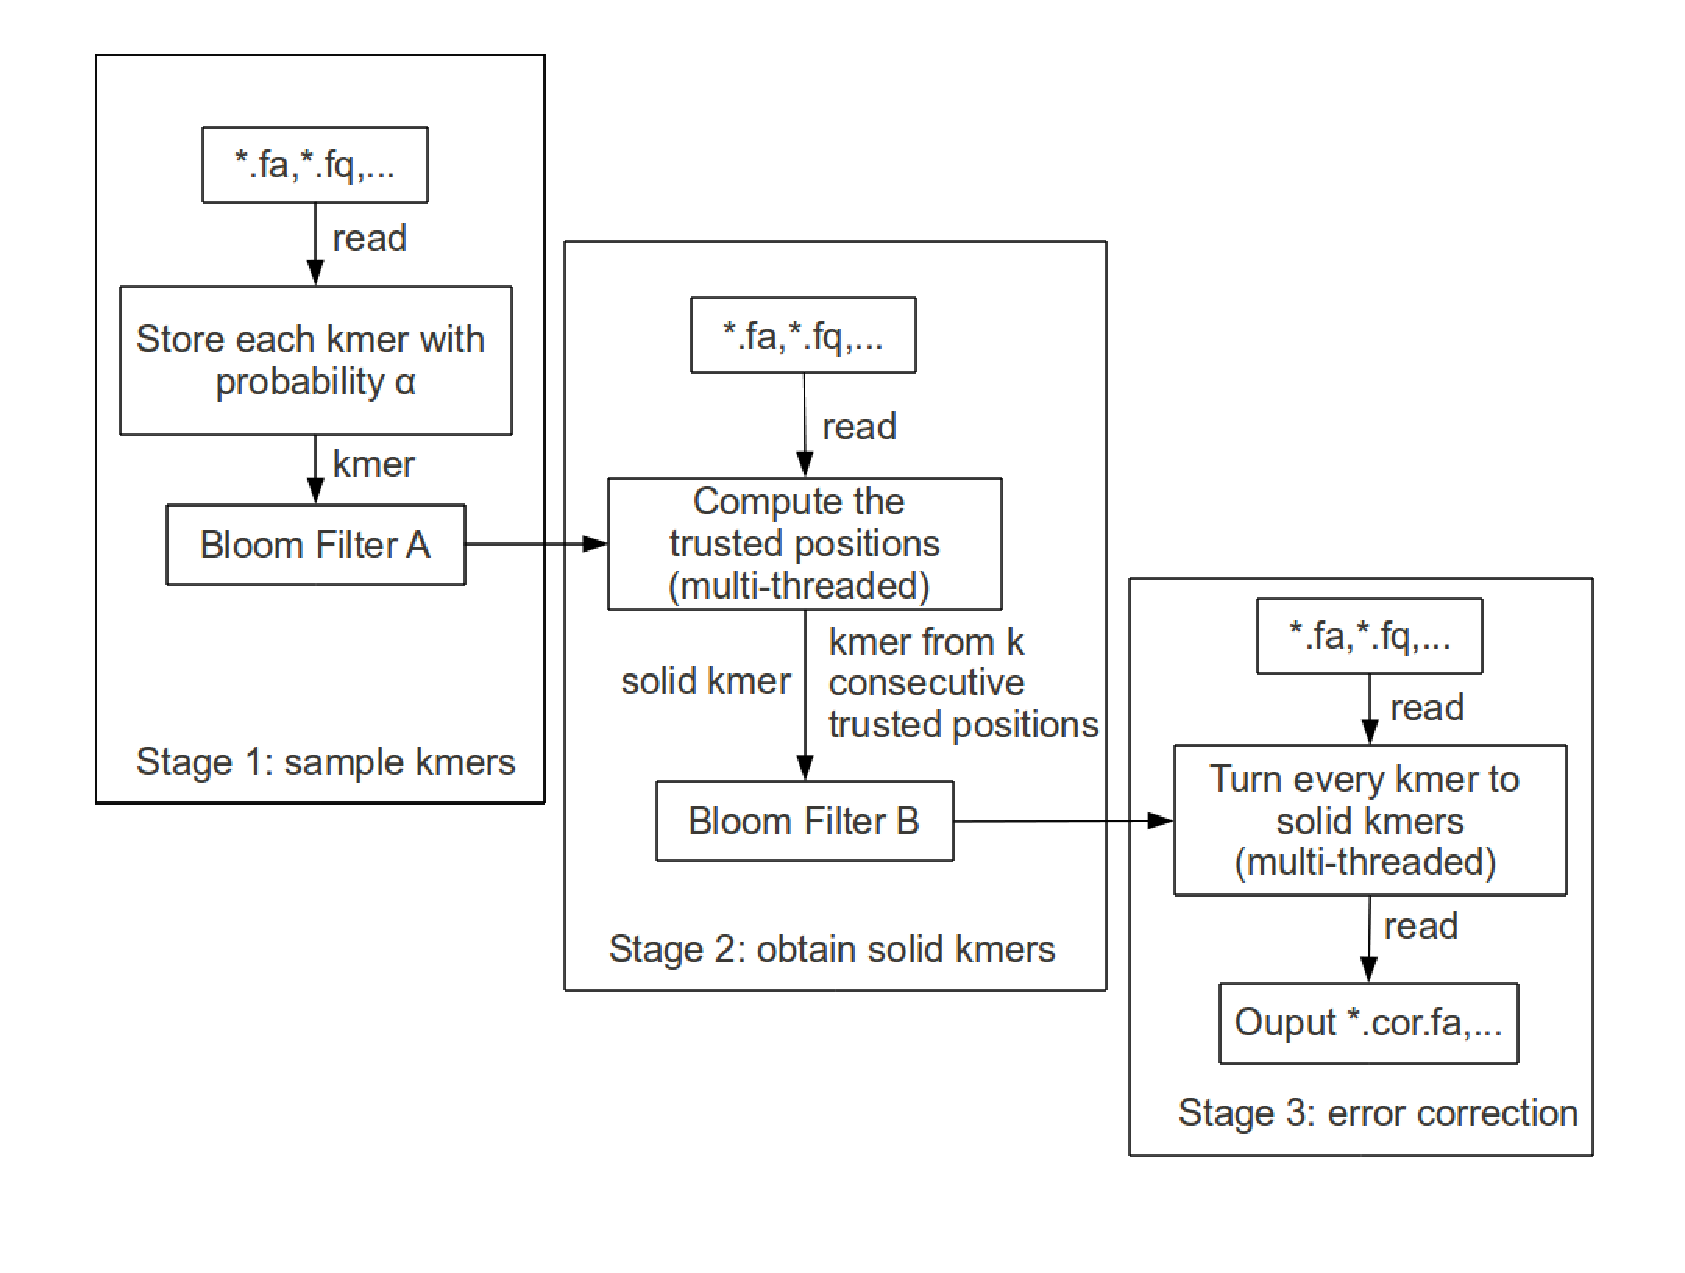
\includegraphics[width=0.75\textwidth]{lighter_framework.eps}
\caption{\csentence{The framework of Lighter}}
\end{figure}

\begin{figure}[h!] %2
\begin{center} 
%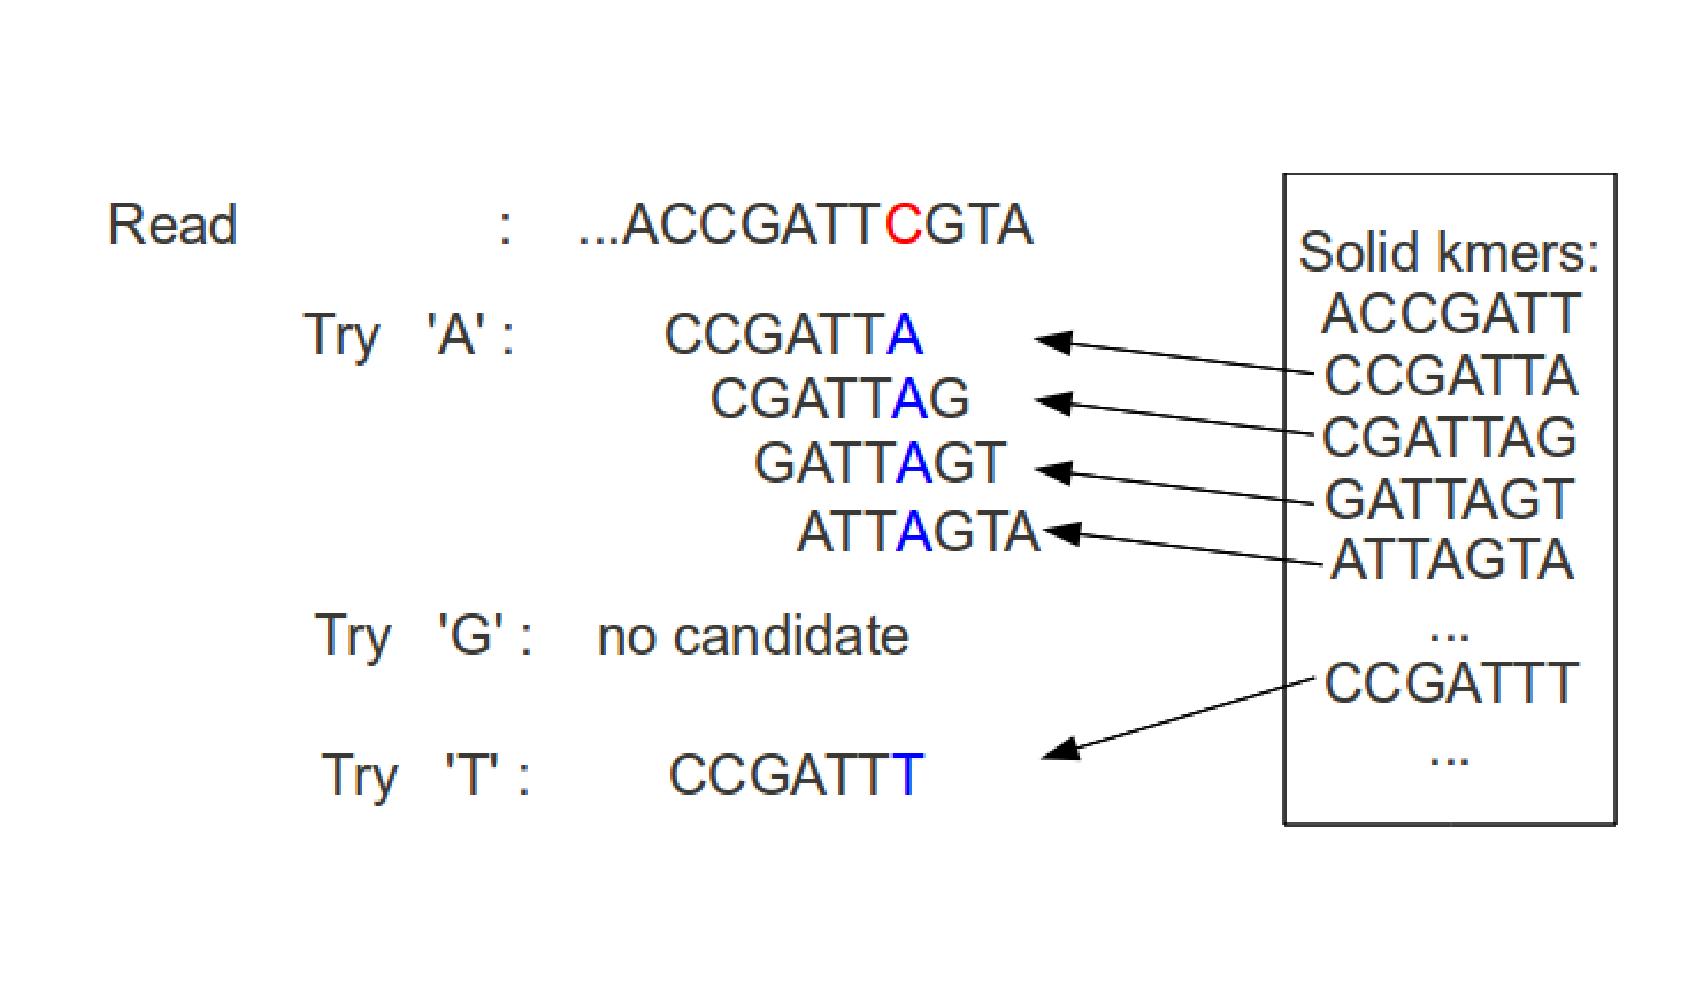
\includegraphics[width=0.75\textwidth]{ErrorCorrection.eps}
\caption{\csentence{An example of the greedy error correction procedure}  \kmer CCGATTC does not appear in Bloom filter $B$, so we attempt to substitute a different nucleotide for the C shown in red.  We select A since it yields the longest stretch of consecutive \kmers that appear in Bloom filter $B$. }
\end{center}
\end{figure}

\begin{figure}[h!] %3
\begin{center}
%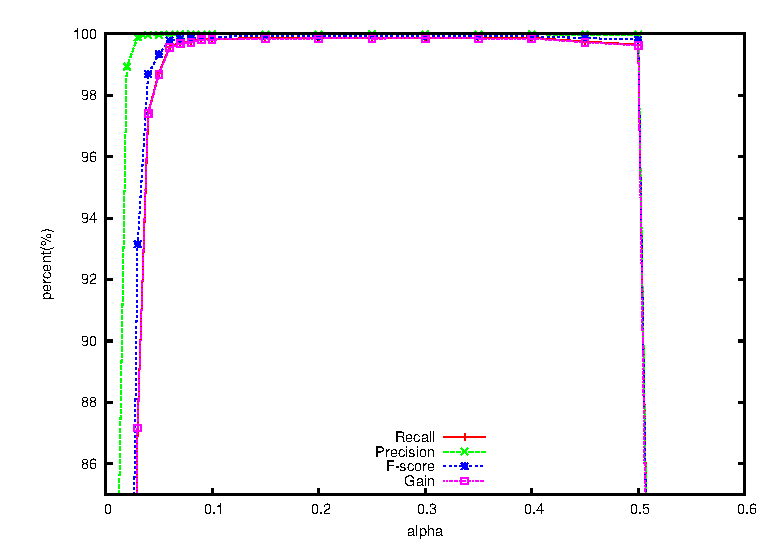
\includegraphics{alpha.eps}
\caption{\csentence{The effect of $\alpha$ on the accuracy using the simulated $35\times$ dataset}}
\end{center}
\end{figure}

\begin{figure}[h!] %4
\begin{center}
%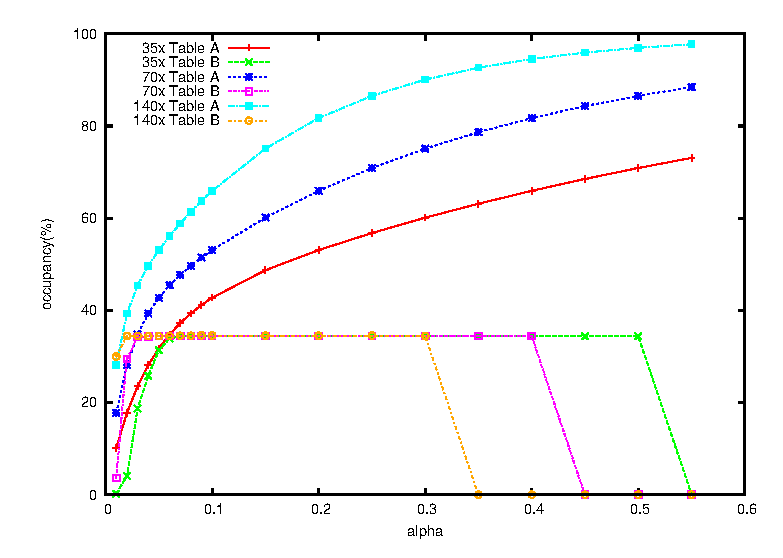
\includegraphics{bloom_occupancy_alpha.eps}
\caption{\csentence{The effect of $\alpha$ on occupancy of Bloom filters $A$ and $B$} The effect of $\alpha$ on occupancy of Bloom filters $A$ and $B$ using simulated $35\times$, $70\times$ and $140\times$ datasets.}
\end{center}
\end{figure}

\begin{figure}[h!] %5
\begin{center}
%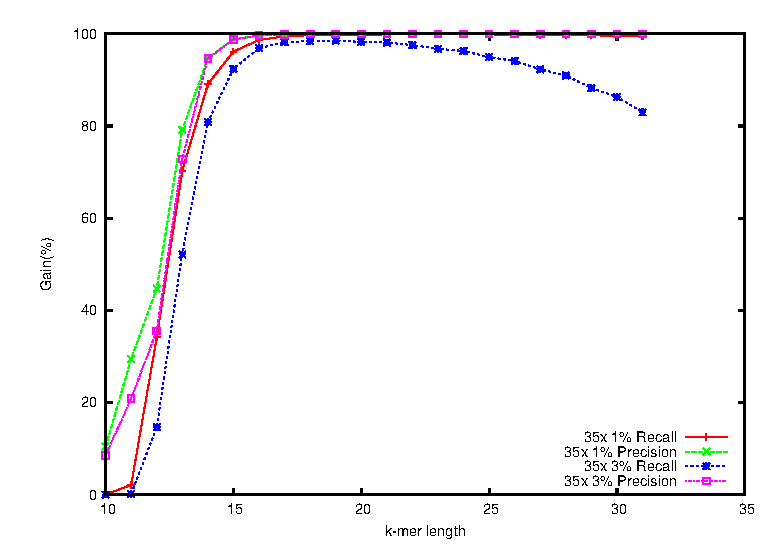
\includegraphics{kmerLength.eps}
\caption{\csentence{The effect of \kmer length $k$ on accuracy}}
\end{center}
\end{figure}

\begin{figure}[h!] %6
\begin{center}
%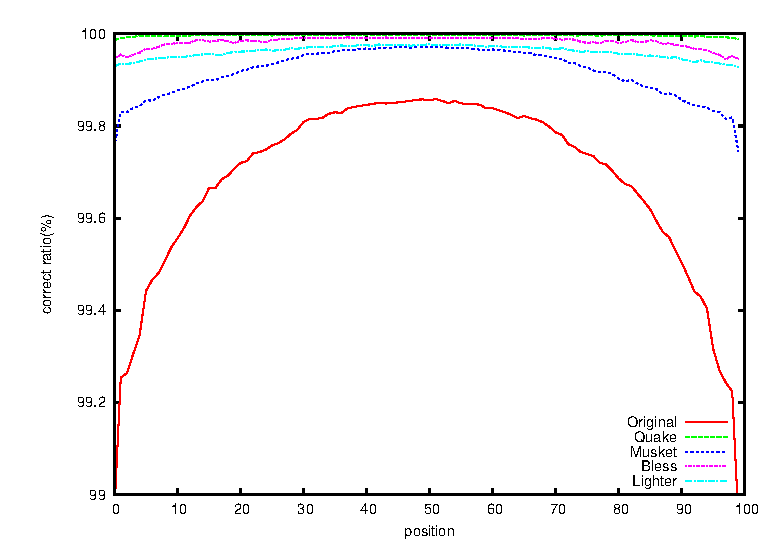
\includegraphics{per_base.eps}
\caption{\csentence{The matching ratio for each base in \ecoli data set}}
\end{center}
\end{figure}

\begin{figure}[h!] %7
\begin{center}
%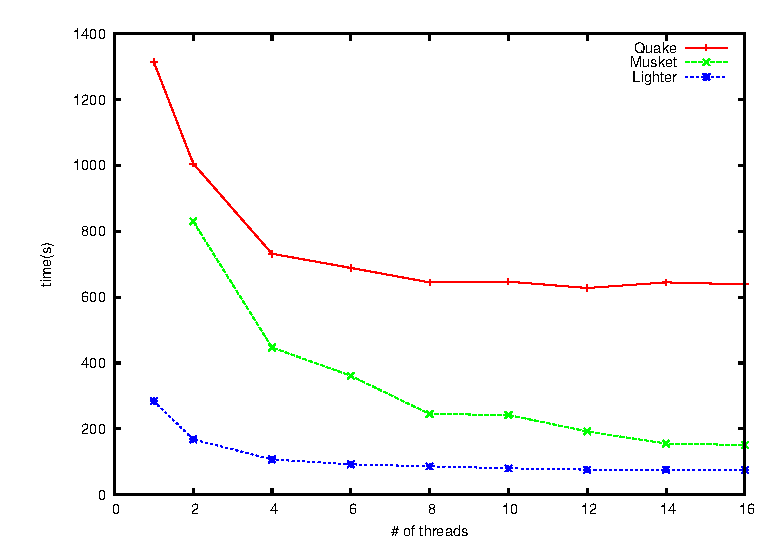
\includegraphics{runtime.eps}
\end{center}
\caption{\csentence{Running times} The running times of Quake, Musket and \tool on $70\times$ simulated data set with increasing number of threads}
\end{figure}

%%%%%%%%%%%%%%%%%%%%%%%%%%%%%%%%%%%
%%                               %%
%% Tables                        %%
%%                               %%
%%%%%%%%%%%%%%%%%%%%%%%%%%%%%%%%%%%

%% Use of \listoftables is discouraged.
%%
\section*{Tables} %1
\begin{table}[h!]
\caption{Accuracy measures for simulated  rate(\%) for each table for different coverages}
\begin{tabular}{|c|c|c|c|c|c|c|c|}\hline
Coverage &	& \multicolumn{2}{|c|}{$35\times$}  & \multicolumn{2}{|c|}{$70\times$} & \multicolumn{2}{|c|}{$140\times$} \\ \hline
Error rate & & $1\%$ & $3\%$ & $1\%$ & $3\%$ & $1\%$ & $3\%$ \\ \hline
$\alpha$ for lighter & & $0.1$ & $0.1$ & $0.05$ & $0.05$ & $0.025$ & $0.025$ \\ \hhline{|=|=|=|=|=|=|=|=|}
	& quake	& 89.59	& 48.77	& 89.64	& 48.82	& 89.59	& 48.78 \\ \cline{2-8}
Recall	& musket	& 92.61	& 92.04	& 92.60	& 92.05	& 92.60	& 92.03 \\ \cline{2-8}
	& bless	& 98.68	& 97.29	& 98.69	& 97.48	& 98.65	& 97.47 \\ \cline{2-8}
	& lighter	& \textbf{99.42}	& \textbf{98.03}	& \textbf{99.36}	& \textbf{98.93} & \textbf{99.39}	& \textbf{98.99} \\ \hhline{|=|=|=|=|=|=|=|=|}
	& quake	&\textbf{99.99}	& \textbf{99.99}	& \textbf{99.99}	& \textbf{99.99}	& \textbf{99.99}	& \textbf{99.99} \\ \cline{2-8}
Precision	& musket	& 99.78	& 99.63	& 99.78	& 99.63	& 99.78	& 99.63 \\ \cline{2-8}
	& bless	& 98.90	& 98.59	& 98.88	& 98.62	& 98.88	& 98.61 \\ \cline{2-8}
	& lighter	& 99.10 & 99.14	& 99.08	& 99.18	& 99.07	& 99.18 \\ \hhline{|=|=|=|=|=|=|=|=|}
	& quake	& 94.51	& 65.56	& 94.54	& 65.61	& 94.51	& 65.57 \\ \cline{2-8}
F-score	& musket	& 96.06	& 95.68	& 96.05	& 95.69	& 96.05	& 95.68 \\ \cline{2-8}
	& bless	& 98.79	& 97.94	& 98.78	& 98.04	& 98.77	& 98.04 \\ \cline{2-8}
	& lighter	& \textbf{99.26}	& \textbf{98.58}	& \textbf{99.22}	& \textbf{99.06}	& \textbf{99.23}	& \textbf{99.09} \\ \hhline{|=|=|=|=|=|=|=|=|}
	& quake	& 89.58	& 48.76	& 89.64	& 48.82	& 89.59	& 48.78 \\ \cline{2-8}
Gain	& musket	& 92.40	& 91.70	& 92.39	& 91.71	& 92.39	& 91.69 \\ \cline{2-8}
	& bless	& 97.58	& 95.90	& 97.57	& 96.11	& 97.54	& 96.09 \\ \cline{2-8}
	& lighter	& \textbf{98.52}	& \textbf{97.17}	& \textbf{98.44}	& \textbf{98.12}	& \textbf{98.46}	& \textbf{98.18} \\ \hhline{|=|=|=|=|=|=|=|=|}

\end{tabular}
\end{table}


\begin{table}[h!] %2
\caption{Occupancy rate(\%) for each table for different coverages}
\begin{tabular}{|c|c|c|c|}\hline
Coverage & $\alpha$ & Bloom $A$ & Bloom $B$ \\ \hline
$10\times$	& 0.35 & 41.563  &	19.843 \\ \hline
$20\times$	& 0.175 & 41.555  &	32.765 \\ \hline
$35\times$ & 0.1 &41.555	& 33.802 \\ \hline
$70\times$ & 0.05 &41.580	& 33.906 \\ \hline
$140\times$ & 0.025 & 41.577 & 33.881  \\ \hline
$280\times$ & 0.0125 & 41.571 & 33.903 \\ \hline
\end{tabular}
\end{table}

\begin{table}[h!] %3
\caption{Alignment statistics for the $75\times$ \ecoli data set, before error correction (Original row) and after error correction (Quake, Musket, BLESS and \tool rows).  The first ``Increase'' column shows percent increase in reads aligned.  The second ``Increase'' column shows percent increase in average number of matching positions per aligned read.}
\begin{tabular}{|c|c|c||c|c|} \hline
	 & \multicolumn{2}{|c||}{Read Level} & \multicolumn{2}{|c|}{Base Level} \\ \hline
     & Mapped Reads & Increase(\%) & Base Match/Read & Increase(\%) \\ \hline
Original & 	3,464,137	 & - & 99.038	& - \\ \hline
Quake	& 3,475,689	& 0.33	& 97.982	& -1.97  \\ \hline
Musket	& 3,467,875	& 0.11	& 99.601	& 0.57  \\ \hline
BLESS	& 3,472,976	& 0.26	& 99.611	& 0.58  \\ \hline
Lighter	&  3,476,422	& 0.35	& 99.611	& 0.58  \\ \hline
\end{tabular}
\end{table}

\begin{table}[h!] %4
\caption{De novo assembly of \ecoli data set}
\begin{tabular}{|c|c|c|c|c|c|} \hline
	 	& N50 &	NG50	 & Edits / 100kbps&	Misassemblies	& Coverage(\%) \\ \hline
Original &	94,879 &	87,008	& 3.41	& 0	& 97.496  \\ \hline
Quake	& 100,379 &	91,194	& 5.6	& 2	 & 97.515  \\ \hline
Musket	& 86,419  &	79,481	& 7.25	& 1	 & 97.504  \\ \hline
BLESS	& 94,879  &	90,126	& 4.72	& 1	& 97.419  \\ \hline
Lighter	& 98,555  &	94,875	& 4.84	& 2	& 97.510  \\ \hline

\end{tabular}
\end{table}


\begin{table}[h!]%5
\caption{Alignment of chr14 data set}
\begin{tabular}{|c|c|c||c|c|}\hline
  & \multicolumn{2}{|c||}{Read Level} & \multicolumn{2}{|c|}{Base Level} \\ \hline
  & Mapped Reads  &Increase(\%) & Base Match/Read	& Increase(\%) \\ \hline
Original & 35,993,146	&- 		&	99.492	& - \\ \hline
Quake 	& 36,164,028	& 0.47 &	92.622	& -6.90 \\ \hline
Musket 	&	36,316,697	& 0.90	& 100.100	& 0.61 \\ \hline
BLESS 	&36,297,285	& 0.84	& 100.192	&	0.70 \\ \hline
Lighter	&36,280,347	& 0.80	& 100.109	& 0.62 \\ \hline
\end{tabular}
\end{table}

\begin{table}[h!] %6
\caption{De novo assembly of chr14 data set}
\begin{tabular}{|c|c|c|c|c|c|} \hline
	   & N50 &	NG50	& Edits / 100kbps &	Misassemblies	& Coverage(\%) \\ \hline
Original &	5277	&3847	&139.16	&1257	&78.777 \\ \hline
Quake	&	4704	&3427	&131.98	&965	&78.55 \\ \hline
Musket	&	5583	&4103	&131.04	&556	&79.175 \\ \hline
BLESS	&	5620	&4114	&128.42	&583	&79.204 \\ \hline
Lighter	&	5712	&4195	&128.92	&544	&79.251 \\ \hline
\end{tabular}
\end{table}

\begin{table}[h!] %7
\caption{Comparison of four error correction tools based on their memory usage (peak resident memory) and disk usage.\label{table:memory_usage}}
\begin{tabular}{|c|c|c||c|c||c|c||c|c|} \hline
		& \multicolumn{2}{|c||}{$35\times$} & \multicolumn{2}{|c||}{$70\times$}  & \multicolumn{2}{|c||}{$140\times$} & \multicolumn{2}{|c|}{chr14}  \\ \hline
		& memory & disk & memory & disk & memory & disk & memory & disk \\ \hline
Quake   & 2.8G	& 3.3G & 7.1G & 6.0G & 14G & 12G & 48G & 57G \\ \hline		
Musket	& 139M	& 0 & 160M & 0 & 241M & 0 & 1.4G & 0 \\ \hline
BLESS	& 10M	& 661M & 11M & 1.3G & 13M & 2.6G & 600M & 15G \\ \hline
Lighter	& 31M	& 0 & 31M & 0 & 31M & 0 & 510M & 0 \\ \hline
\end{tabular}
\end{table}

\end{backmatter}
\end{document}






